\section{Конструкторская часть}

\subsection{Архитектура приложения}

В состав разрабатываемого программного обеспечения входит один загружаемый модуль ядра, который предоставляет пользователю информацию о загруженности оперативной памяти -- ее общее количество, а также количество занятой, свободной и доступной оперативной памяти в данный момент времени.

\subsection{Базовые структуры}

В листингах \ref{lst:procops}-\ref{lst:memstruct} представлены объявления структур struct proc\_ops для работы с виртуальной файловой системой /proc и struct mem\_struct для хранения информации о памяти.

\begin{lstlisting}[label={lst:procops}, caption={структура struct proc\_ops}]
	static const struct proc_ops mem_ops = {
		proc_read: seq_read,
		proc_open: proc_memory_open,
		proc_release: proc_release,
	};
\end{lstlisting}

\begin{lstlisting}[label={lst:memstruct}, caption={структура struct mem\_struct}]
	typedef struct mem_struct {
		long available;
		long free;
		long time_secs;
	} mem_info_t;
\end{lstlisting}

Для использования структуры mem\_ops необходимо реализовать функции proc\_memory\_open() и proc\_release().

\subsection{Разработка алгоритма}

На рисунках \ref{fig:idef_general}-\ref{fig:idef_detailed} представлены IDEF0-диаграммы алгоритма работы программы.

\begin{figure}[h!]
	\begin{center}
		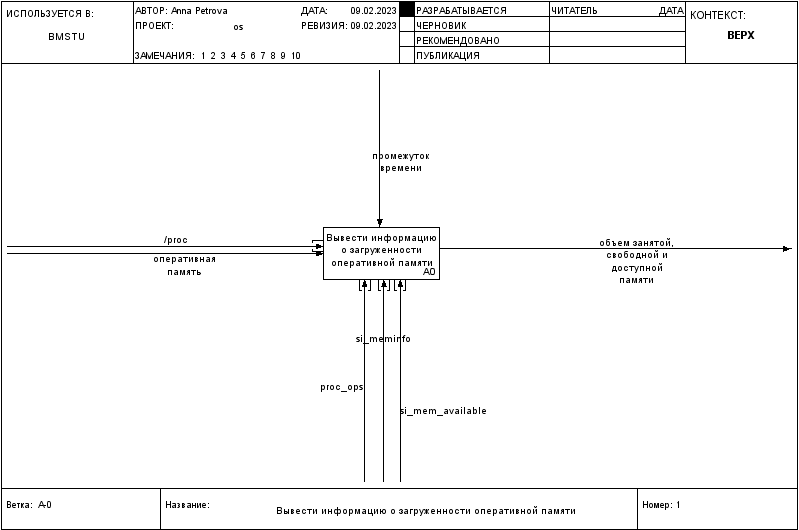
\includegraphics[scale=0.55]{jpg/01_A-0.png}
	\end{center}
	\captionsetup{justification=centering}
	\caption{Общая схема работы}
	\label{fig:idef_general}
\end{figure}

\begin{figure}[h!]
	\begin{center}
		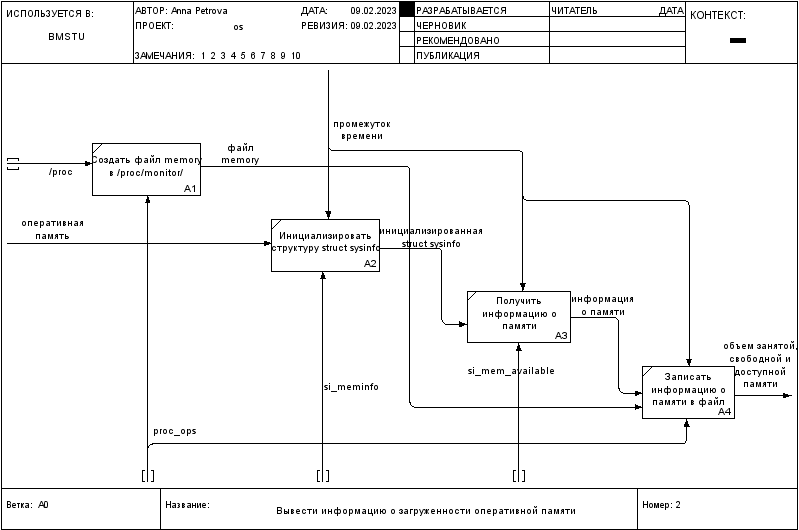
\includegraphics[scale=0.55]{jpg/02_A0.png}
	\end{center}
	\captionsetup{justification=centering}
	\caption{Декомпозиция алгоритма}
	\label{fig:idef_detailed}
\end{figure}

\newpage

\subsection*{Выводы}

В данном разделе была рассмотрена общая архитектура приложения, базовые структуры, необходимые для разработки, а также были приведены IDEF0-диаграммы алгоритма работы программы.

